\documentclass[12pt, titlepage]{report}
\usepackage{consumer_resource_final}
\graphicspath{{./figures/}}

\begin{document}


\subsection{LRI regime}
\subsubsection{Monte Carlo algorithm for the optimal syntrophy matrix} \label{section : numerical analysis LRI MC solver}
We want to find a general algorithm which, for a given food consumption adjacency matrix $G$ gives back an optimal syntrophy adjacency matrix $A$. Strategically, we would like an $A$ such that Eq.\eqref{eq : LRI metaparams sufficient} is as close to being satisfied as possible. If it were satisfied, it would put the system in an LRI regime, which we have proven is dynamically stable.

One way of trying to satisfy Eq.\eqref{eq : LRI metaparams sufficient} is to increase the magnitude of its LHS and minimize the magnitude of the RHS. The LHS is minimized if $(AG)_{\mu\mu}$ is set to its lowest possible value for every $\mu$, that is zero. On the other hand, the RHS is minimized if $\alpha_0(AG)_{\mu\nu}\approx\gamma_0R_0 (G^TG)_{\mu\nu} \ \forall \nu\neq\mu$.

Intuitively, we then search for systems where $AG$ is zero on the diagonal, \ie where no coprophagy is observed, and $AG \approx \frac{\gamma_0R_0}{\alpha_0}G^TG$ outside the diagonal. It can be formalized by writing a proper Metropolis-Hastings Markov Chain Monte Carlo (MCMC) method. We designed the following algorithmic procedure to build a syntrophy adjacency matrix $A$:
\begin{enumerate}
\item Create a random $A$. Its connectance is chosen as the one of the consumption matrix $G$.
\item Do the following for a given number of steps:
\begin{itemize}
\item Choose a random row or, every other iteration, a column.
\item In that row/column, try to swap a zero and a one while preserving the ``releasers'': if a species releases some resource, it has to keep releasing something (the resource can change though). The ``releasees'' are preserved as well : if a resource is being released by some species, it has to keep being released (but it does not have to be by the same species). \textbf{why do we impose those conditions?}
\item The swap is accepted, \ie $A$ is modified, if the energy difference $\Delta E$ is negative or if a random number drawn uniformly between zero and one is smaller than $e^{-\Delta E/T}$ where $T$ is the current temperature. More on $\Delta E$ and $T$ below.
\end{itemize}
\item Return $A$.
\end{enumerate}
A couple comments on this algorithm can be made:
\begin{itemize}
\item The algorithm preserves the connectance of $A$ but not its nestedness. The question of what value to choose is open, but we choose $\kappa(A)=\kappa(G)$ as a first approach, \ie syntrophy and consumption networks have the same connectance.
\item The temperature $T$ changes dynamically during the simulation. It is obtained in a way close to the spirit of simulated annealing techniques \cite{gendreau_simulated_2019} : the temperature $T$ is multiplied by a factor $\lambda=0.99$ at a fixed frequency (for instance every 1000 steps). We add the requirement that if new moves are rejected during too many consecutive steps, we multiply the temperature by $1/\lambda$.
\item The energy difference $\Delta E$ between the new proposed $A'$ and the old $A$ is computed by assigning an energy $E$ to both $A'$ and $A$ and subtracting them:
\begin{equation}
\Delta E \defined E(A')-E(A).
\end{equation}
The choice of the energy function $E$ is crucial. In essence, this MCMC algorithm will find the specific $A$ which minimizes $E(A)$. Since we want to work with systems in the LRI regime, we use the simplest and most natural function that is compatible with the intuitively expected characteristics of $A$ explained above (\ie $AG$ is zero on the diagonal and equal to $\frac{\gamma_0 R_0}{\alpha_0} G^TG$ outside of it):
\begin{equation}
E(A) \defined \sum_\mu \left( \abs{\alpha_0(AG)_{\mu\mu}} + \sum_{\nu\neq\mu} \abs{(\alpha_0 AG-\gamma_0 R_0 G^TG)_{\mu\nu} }\right).
\end{equation}
The energy function and hence the optimal syntrophy adjacency matrix $A$ depend on the ratio $\frac{\alpha_0}{\gamma_0 R_0}$. This prompts then the question of which $\alpha_0$ can be deemed sensible. As a first step, we will take the value of Eq.\eqref{eq : largest feasible alpha0} : $\alpha_0 = \min(1-\sigma_0, \sigma_0) \gamma_0 R_0 N_R$. This means that the outcome of the algorithm is an optimized $A$ \textbf{for the largest feasible syntrophy}. Since the expression we have for the largest feasible syntrophy is independent of the $G$ matrix, this choice of $\alpha_0$ provides us a sensible way of comparing different consumption networks.
\end{itemize}




\subsection{The effect of sigma non uniform}
\begin{figure}
\includegraphics[width=0.6\linewidth]{figures/eigenvalues_Nest015_Conn01808_sigma_uniform}
\caption{Eigenvalues $\kappa=0.1808$, $\eta=0.15$, $R_0=\gamma_0=0.2$, $\alpha_0=0$, $\sigma_0=0.25$, uniform efficiency matrix (Butler case).}
\includegraphics[width=0.6\linewidth]{figures/eigenvalues_Nest015_Conn01808_sigma_spread}
\caption{Eigenvalues $\kappa=0.1808$, $\eta=0.15$, $R_0=\gamma_0=0.2$, $\alpha_0=0$, $\sigma_0=0.25$, efficiency matrix with a spread. We observed some systems with an eigenvalue larger than zero.}
\end{figure}

\subsection{Time evolution}
\begin{figure}[h!]
\centering
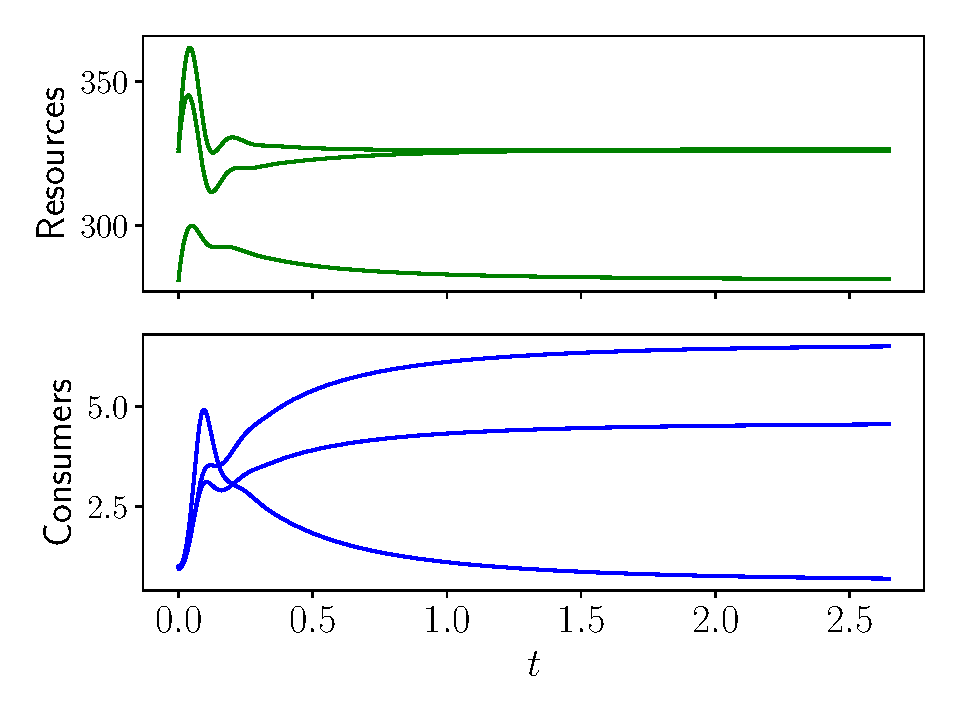
\includegraphics[width=0.6\linewidth]{Typical_time_evolution/Typical_time_evolution_resources_species_high_threshold.pdf}
\caption{Time evolution for high coefficient threshold ($\epsilon_{\text{conv}}=10^{-1}$)}
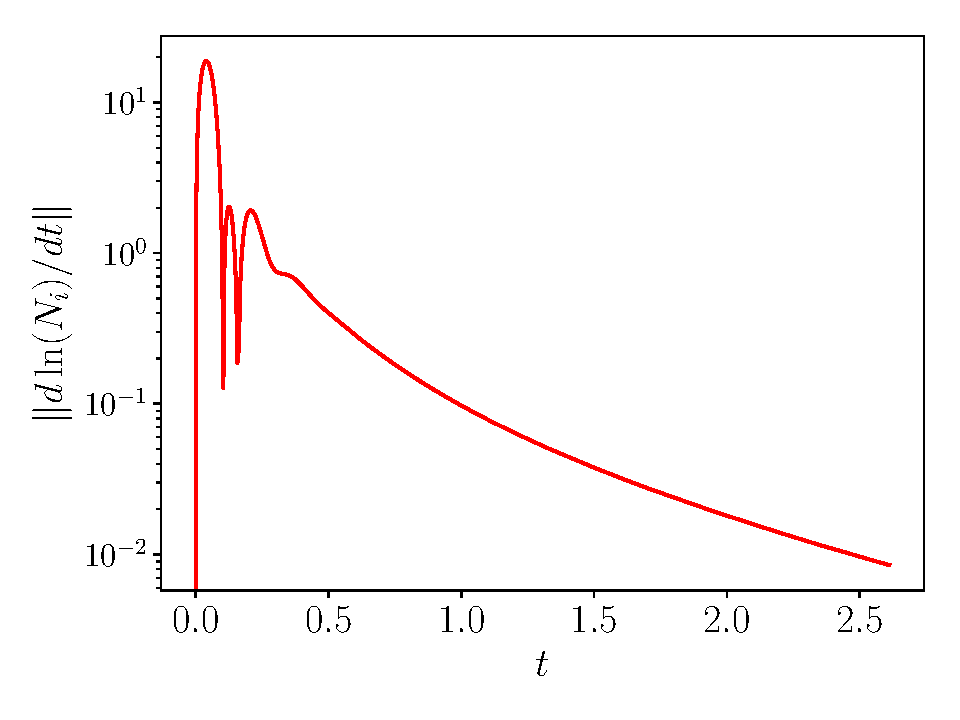
\includegraphics[width=0.6\linewidth]{figures/Typical_time_evolution/Typical_time_evolution_log_derivative_high_threshold.pdf}
\caption{Typical convergence to judge equilibrium, we see the simulation stops at $\epsilon_{\text{conv}}=10^{-1}$}
\end{figure}
\begin{figure}[h!]
\centering
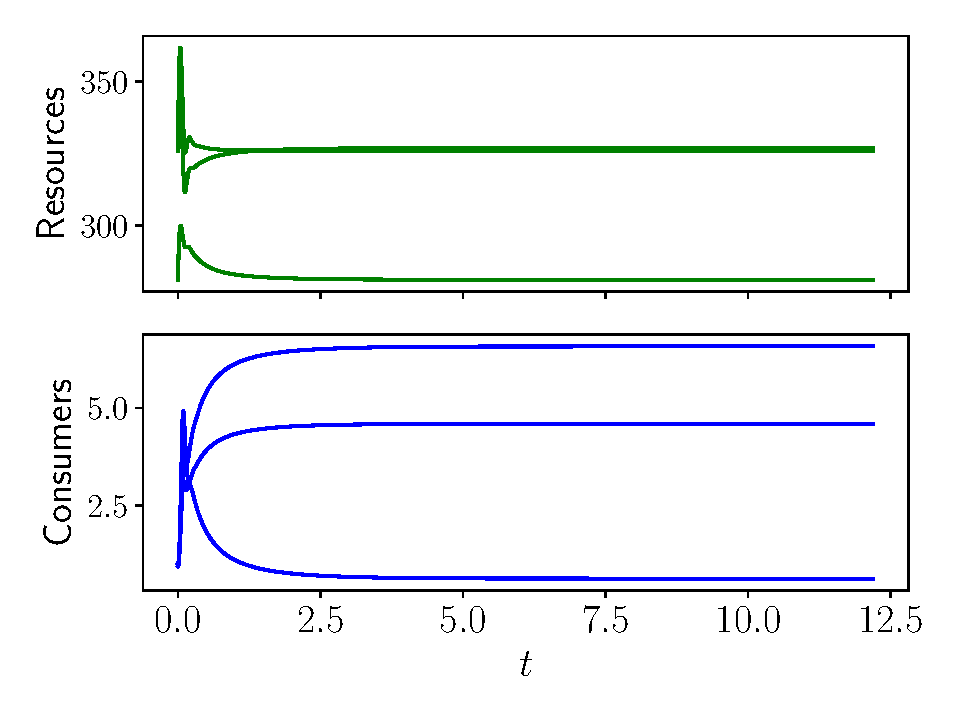
\includegraphics[width=0.6\linewidth]{Typical_time_evolution/Typical_time_evolution_resources_species_low_threshold.pdf}
\caption{Time evolution for low coefficient threshold (more accuracy) ($\epsilon_{\text{conv}}=10^{-5}$)}
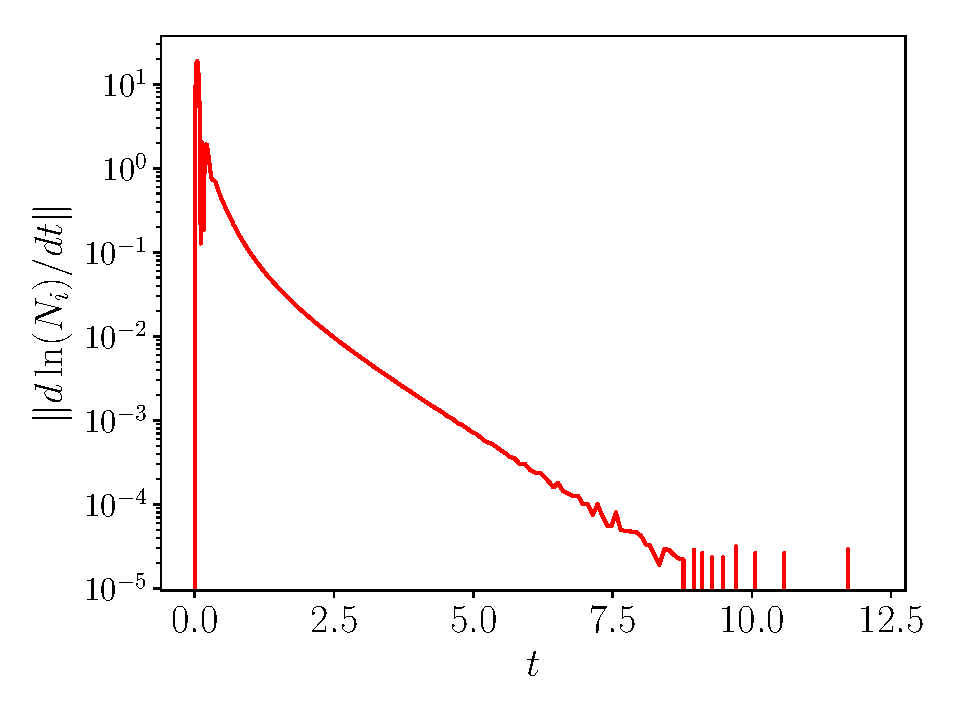
\includegraphics[width=0.6\linewidth]{figures/Typical_time_evolution/Typical_time_evolution_log_derivative_low_threshold.pdf}
\caption{Typical convergence to judge equilibrium, we see the simulation stops at $\epsilon_{\text{conv}}=10^{-5}$}
\end{figure}
\subsection{Allowed parameters : syntrophy range}
\begin{figure}[h!]
\centering
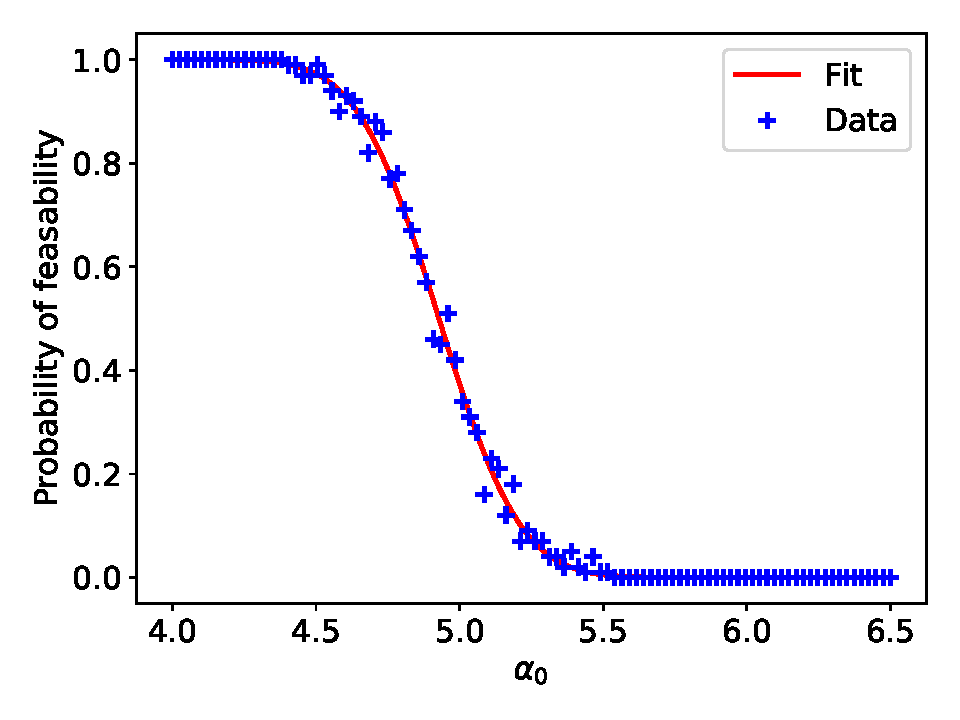
\includegraphics[scale=0.7]{figures/alpha0_probability_of_feasability}
\caption{Typical shape of the probability of feasability for every metaparameter fixed except varying $\alpha_0$. We see that the probability of drawing a feasible system decreases sharply as $\alpha_0$ increases. A typical sigmoidal curve (here an erf function) fits the numerical data quite well.}
\end{figure}

\subsection{Studying the impact of the food network structure}
\subsection{Studying the impact of syntrophy}
We run a bunch of simulations with the following metaparameters. We made sure that these are compatible with the bounds on $\alpha_0$ Eqs.\eqref{eq : alpha bounds}.

% Please add the following required packages to your document preamble:
% \usepackage{graphicx}
\begin{table}[h!]
\centering
\begin{tabular}{c|c|c|c|c|c}
$\gamma_0$ & $\sigma_0$ & $\alpha_0$ & $R_0$ & $S_0$ & $l_0$ \\ \hline
1          & 1          & 0          & 300   & 1     & 11091 \\
         & 0.75       & 0          &       &       &       \\
         &            & 0.5        &       &       &       \\
         & 0.5        & 0          &       &       &       \\
         &            & 0.5        &       &       &       \\
         &            & 1          &       &       &       \\
         & 0.25       & 0          &       &       &       \\
         &            & 0.5        &       &       &       \\
         &            & 1          &       &       &       \\
         &            & 1.5        &       &       &
\end{tabular}
\caption{Metaparameters used for the simulations.} \label{eq : table metaparameters used}
\end{table}

\end{document}
